\documentclass[a4paper,12pt]{article}
\usepackage{setspace}
\usepackage{sectsty}
\usepackage{siunitx}
\usepackage{graphicx}
\usepackage[a4paper, total={3in, 9in}, textwidth=16cm,bottom=1in,top=1.4in]{geometry}
\usepackage[dvipsnames]{xcolor}
\usepackage{amsmath}
\usepackage{esvect}
\usepackage{soul}
\usepackage{amsthm}
\usepackage{hyperref}
\usepackage{longtable}
\usepackage{float}
\usepackage{amssymb}
\usepackage{outlines}
\usepackage{caption}
\usepackage{fancyvrb}
\usepackage{subcaption}
\usepackage{esdiff}
\usepackage{dirtytalk}
\usepackage{colortbl}
\usepackage{booktabs}
\usepackage{setspace}
\usepackage{mathtools}
\usepackage{tikz,pgfplots}
\usepackage[most]{tcolorbox}
\usepackage{draftwatermark}
\usepackage{helvet}
\renewcommand{\familydefault}{\sfdefault}
\SetWatermarkText{timthedev07}
\SetWatermarkScale{4}
\SetWatermarkColor[gray]{0.97}
\usetikzlibrary{positioning,decorations.markings,arrows.meta,angles,quotes}
\DeclarePairedDelimiter{\ceil}{\lceil}{\rceil}
\newtheorem{lemma}{Lemma}
\newtheorem{proposition}{Proposition}
\newtheorem{remark}{Remark}
\newtheorem{observation}{Observation}
\doublespacing
\let\oldsection\section
\renewcommand\section{\clearpage\oldsection}
\newcommand{\RNum}[1]{\uppercase\expandafter{\romannumeral #1\relax}}
\let\oldsi\si
\renewcommand{\si}[1]{\oldsi[per-mode=reciprocal-positive-first]{#1}}
\usepackage{enumitem}
\newcommand{\subtitle}[1]{%
  \posttitle{%
    \par\end{center}
    \begin{center}\large#1\end{center}
    \vskip0.5em}%
}
\newcommand{\degsym}{^{\circ}}
\newcommand{\Mod}[1]{\ (\mathrm{mod}\ #1)}
\usepackage{hyperref}
\hypersetup{
  colorlinks=true,
  linkcolor = blue
}
\newcommand{\lb}{\\[8pt]}
\newenvironment*{cell}[1][]{\begin{tabular}[c]{@{}c@{}}}{\end{tabular}}
\newcommand{\img}[4]{\begin{center}
  \begin{figure}[H]
    \centering
    \includegraphics[width=#2\textwidth]{#1}
    \caption{#3}
    \label{fig:#4}
  \end{figure}
\end{center}}
\parindent=0pt
\usepackage{fancyhdr}
\fancyfoot{}
\fancypagestyle{fancy}{\fancyfoot[R]{\vspace*{1.5\baselineskip}\thepage}}
\renewcommand{\contentsname}{Table of Contents}
\newcommand{\angled}[1]{\langle{#1}\rangle}
\newcommand{\paren}[1]{\left(#1\right)}
\newcommand{\sqb}[1]{\left[#1\right]}
\newcommand{\coord}[3]{\angled{#1,\, #2,\, #3}}
\newcommand{\pair}[2]{\paren{#1,\, #2}}
\newcommand{\atom}[3]{{}^{#1}_{#2}\text{#3}}
\usepackage[
  noabbrev,
  capitalise,
  nameinlink,
]{cleveref}

\crefname{lemma}{Lemma}{Lemmas}
\crefname{proposition}{Proposition}{Propositions}
\crefname{remark}{Remark}{Remarks}
\crefname{observation}{Observation}{Observations}

\newtcolorbox[auto counter]{prob}[2][]{fonttitle=\bfseries, title=\strut Problem~\thetcbcounter: #2,#1,colback=Orchid!5!white,colframe=Orchid!75!black,top=5mm,bottom=5mm}

\newtcolorbox[auto counter]{rem}[1][]{fonttitle=\bfseries, title=\strut Remark.~\thetcbcounter,colback=purple!5!white,colframe=purple!65!gray,top=5mm,bottom=5mm}

\newtcolorbox[auto counter]{defin}[1][]{fonttitle=\bfseries, title=\strut Definition.~\thetcbcounter,colback=black!5!white,colframe=black!65!gray,top=5mm,bottom=5mm}

\newtcolorbox[auto counter]{obs}[1][]{fonttitle=\bfseries, title=\strut Observation.~\thetcbcounter,colback=RedViolet!5!white,colframe=RedViolet!65!gray,top=5mm,bottom=5mm}

\newtcolorbox[auto counter]{lem}[1][]{fonttitle=\bfseries, title=\strut Lemma.~\thetcbcounter,colback=Maroon!5!white,colframe=Maroon!65!gray,top=5mm,bottom=5mm}

\newtcolorbox[auto counter]{prop}[1][]{fonttitle=\bfseries, title=\strut Proposition.~\thetcbcounter,colback=RedOrange!5!white,colframe=RedOrange!65!gray,top=5mm,bottom=5mm}

\newtcolorbox[auto counter]{hint}[1][]{fonttitle=\bfseries, title=\strut Hint.~\thetcbcounter,colback=OliveGreen!5!white,colframe=OliveGreen!75!gray,top=5mm,bottom=5mm}

\setlength{\belowcaptionskip}{-20pt}
\begin{document}


\pagenumbering{arabic}
\pagestyle{fancy}


\begin{titlepage}
  \begin{center}

    \vspace*{8cm}
    \textbf{\Large {IB Physics Topic E5 Fusion and Stars; SL \& HL}} \\
    \vspace*{1cm}
    \large{By timthedev07, M25 Cohort}

  \end{center}
\end{titlepage}

\pagebreak
\tableofcontents
\pagebreak

\clearpage
\setcounter{page}{1}
\addtocontents{toc}{\protect\thispagestyle{empty}}

\section{Fusion in Stars}

Conditions for proton-proton cycle and thus hydrogen fusion to occur:
\begin{itemize}
  \item High temperature: to overcome the electrostatic repulsion between the nuclei
  \item High pressure: to overcome the gravitational attraction between the nuclei
\end{itemize}

The hydrogen fusion has three stages
\begin{enumerate}
  \item \textbf{Proton-proton reaction}: Two protons (hydrogen nuclei) collide at extremely high temperatures and pressures, fusing together to form a \textit{deuterium nucleus} (one proton and one neutron), releasing a positron and a neutrino, while converting a proton into a neutron via beta-plus decay.
        \[
          \atom{1}{1}{H} + \atom{1}{1}{H} \rightarrow \atom{2}{1}{H} + \atom{0}{1}{$\beta$}^{+} + \nu_e
        \]
  \item \textbf{Deuterium-proton reaction}: The newly formed deuterium nucleus fuses with another proton, resulting in a helium-3 nucleus (two protons and one neutron). This releases a gamma ray.
        \[
          \atom{2}{1}{H} + \atom{1}{1}{H} \rightarrow \atom{3}{2}{He} + \gamma
        \]
  \item \textbf{Helium-3 fusion}: Two helium-3 nuclei from stage 2 fuse to form a helium-4 nucleus (two protons and two neutrons) while releasing two protons. This stage releases about 12.9 MeV of energy.

        \[
          \atom{3}{2}{He} + \atom{3}{2}{He} \rightarrow \atom{4}{2}{He} + 2\atom{1}{1}{H}
        \]
\end{enumerate}

\pagebreak

The overall reaction is written as
$$4\atom{1}{1}{H} \rightarrow \atom{4}{2}{He} + 2\atom{1}{1}{H} + 2\atom{0}{1}{$\beta$}^{+} + 2\nu_e + \gamma$$
\text{or equivalently}
$$2\atom{1}{1}{H} \rightarrow \atom{4}{2}{He} + 2\atom{0}{1}{$\beta$}^{+} + 2\nu_e + \gamma$$


The difficulties of using fusion to produce energy include:
\begin{itemize}
  \item Requires high pressure and temperature
  \item Reactants must overcome Coulomb/intermolecular repulsion
  \item Difficult to contain and control at high temperatures
  \item Difficult to capture energy from fusion reactions
  \item Difficult to maintain/sustain a constant reaction rate
\end{itemize}

Advantages of using fusion to produce energy include:
\begin{itemize}
  \item Plentiful fuel supplies
  \item Larger specific energy
  \item Larger energy density
  \item Little or no major radioactive waste products
\end{itemize}

\section{HR Diagrams}

By the Stefan-Boltzmann law, large stars with high temperatures must be bright. The pattern of stars can be shown on a scatter plot of luminosity against surface temperature; this is known as the Hertzsprung-Russell (HR) diagram.

Notes about the diagram:
\begin{itemize}
  \item The plot is logarithmic on both axes.
  \item The log. temperature ($x$) axis is plotted in decreasing order from left to right.
  \item The log. luminosity ($y$) axis is plotted in increasing order from bottom to top.
  \item An alternative $x$-axis is the spectral class, which is another measure of the temperature of the star.
  \item Each of the lines in \cref{fig:HR} represents a set of stars with the same radius: By the Stefan-Boltzmann law, \hl{$L = 4\pi\sigma R^2T^4$}; for a constant radius, $L\propto T^4$ and on a log-log plot, this is $\ln L \propto \ln T$, a linear relationship.
\end{itemize}

\begin{minipage}{0.5\textwidth}
  \img{hr1.png}{1}{Principle regions and lines of equal radii}{HR}
\end{minipage}%
\begin{minipage}{0.5\textwidth}
  \img{hr2.png}{1}{Scatter plot}{HR2}
\end{minipage}%

\pagebreak

Components of the graph:
\begin{enumerate}
  \item The blue area highlights the region of \textbf{main sequence} stars; this contains 90\% of all stars.
  \item \textbf{Red giants} are cooler than the Sun but have a larger radius. Although they emit less energy per unit area, their combined area is larger, making them equally bright as some main-sequence stars.
  \item \textbf{Supergiants} are brighter than most main sequence stars and very large. Some of them emit $10^5$ times the energy of the Sun, and thus have a S.A. $10^5$ times that of the Sun. This means the radius is $\sqrt{10^5}$ times that of the Sun.

        Together with the red giants, these only constitute 1\% of all stars; they have a much shorter lifetime in comparison to the main-sequence.
  \item \textbf{White dwarfs}: The residue of old stars that are extremely hot and dense but have a small radius and a low luminosity. They make up about 9\% of all stars. They take billions of years to cool.
  \item \textbf{The instability strip}: Indicated by the almost vertical gray line in \cref{fig:HR}. Stars above the mass of the Sun enter this region when they reach the end of the main sequence lifetime, become unstable, and pulsate, changing their size cyclically (alternating between increasing and decreasing). Thus, their luminosity varies too.
\end{enumerate}

\subsection{Note on Notation}

The subscript $\odot$ denotes the value of this particular variable of the Sun. For example, $L_{\odot}$ is the luminosity of the Sun, $R_{\odot}$ is the radius of the Sun, $T_{\odot}$ is the temperature of the Sun, and $M_{\odot}$ is the mass of the Sun.

\section{Stellar Evolution}

\subsection{Birth of Stars}

The \textit{stellar medium} is the region of space between stars that contains gas (mainly hydrogen and helium) and dust (mostly carbon and silicon). At a cool temperature, the density of this medium is as low as $10^{-4}$ ions$/$cm$^3$. This is better than any achievable vacuum on Earth.

A gas cloud of the \textbf{stellar medium} is compressed by gravity and the cloud begin to increase in temperature and pressure. This is because the GPE of particles is released and transferred to their thermal energy. The cloud becomes a \textbf{protostar}.

Later, the star enters the HR-diagram from the right-most side, as a \textbf{main sequence star}.

\subsection{Main Sequence}

During the stability period as a main sequence star, the star is in \textbf{hydrostatic equilibrium}, where the inward gravitational force is balanced by the outward thermal \& radiation pressure force. The star is stable and does not change in size. The \textbf{greater the mass} of the star, the \textbf{greater both forces} are. At this stage, the \hl{core is composed mostly of hydrogen}, and the \hl{outer layer is composed of helium}, which is produced by the fusion of hydrogen.
The above suggests that the \textbf{luminosity} of the star has a positive correlation with the \textbf{mass} of the star.
\begin{enumerate}
  \item For a more massive star, the core temperature must be higher to produce a higher pressure, balancing the higher gravitational force.
  \item The higher core temperature results in a higher rate of fusion, producing more energy.
\end{enumerate}

\pagebreak

By the theory of nuclear physics, if $T$ is the lifetime of the star and $M$ is the mass of the star, then
$$T\propto M^{-2.5}$$

Thus, one can conclude the following

\begin{center}
  \textit{The larger the mass, the shorter the time the star remains on the main sequence.}
\end{center}

Approaching the end of the main sequence, the star begins to \textbf{run out of hydrogen} fuel, as most have been turned into helium and no longer available for fusion. The outward pressure decreases --- the forces are now unbalanced and the star \textbf{begins to shrink} due to the stronger gravitational force. The core temperature increases, and the outer layers expand, cooling down and turning red. The star becomes a \textbf{red giant} or a \textbf{supergiant}, depending on the mass of the star.



\subsection{Stellar Evolution of Low-Mass Stars}

This includes those with mass $M < 4M_{\odot}$.
\img{lowmass1.png}{1}{Stellar evolution of low-mass stars}{lowmass1}
\begin{enumerate}
  \item Due to having lower masses, the core of these stars do not suffice for fusion of any product beyond carbon. When the helium in the core is exhausted, the core contracts as it continues to emit radiation.
  \item A double shell forms around the core: An inner shell of helium and an outer shell of hydrogen. The outer shell of hydrogen begins to fuse, causing the star to expand and cool down, becoming a \textbf{red giant}. In this form, \hl{the primary energy source is the fusion of helium in the core}.
  \item As the outer shell expands away from the core, a \textbf{planetary nebula} is formed. The core then further contracts; it will shrink to the size of the Earth, containing ions together with a degenerate electron gas.
  \item At this stage, the core cannot shrink further. The electron gas exerts a pressure called the \textbf{electron degeneracy pressure}, which prevents the star from further collapsing. The star is now a \textbf{white dwarf}.
\end{enumerate}

\img{lowmass.png}{1}{Stellar evolution of low-mass stars}{lowmass}

\pagebreak

\subsection{Stellar Evolution of Large-Mass Stars}

This includes those with mass $M > 4M_{\odot}$.
\begin{enumerate}
  \item In the giant stage, the higher temperature and pressure create elements heavier than carbon.
  \item The giant phase ends when the star has a layered structure (like an onion), with iron ash in the center. The inner layers have elements with higher proton numbers --- i.e. the proton number decreases as we move outwards.
  \item Similar to low-mass stars, the core contracts; but it does not reach stability due to the higher mass.
  \item The \textbf{Chandrasekhar limit} predicts that stars with a remnant mass above 1.4 M$_{\odot}$ cannot turn into white dwarfs.
  \item As the core continue to contract, electrons and protons combine to form neutrons, releasing neutrinos.
  \item Both the cores and outer layers of the star rapidly collapse, causing a huge explosion known as a \textbf{supernova}.
  \item After the explosion, the outer layers are blown away, leaving only the core, small but extremely dense. Two outcomes are possible from this point
        \begin{enumerate}
          \item The core remains as a \textbf{neutron star}. By the Oppenheimer-Volkoff limit, the mass of a neutron star is limited to 2-3 M$_{\odot}$. Beyond this limit, the core collapses further into a black hole.
          \item The core collapses further, forming a \textbf{black hole}.
        \end{enumerate}
\end{enumerate}

\img{highmass.png}{1}{Stellar evolution of high-mass stars}{highmass1}

\subsubsection{Detecting Black Holes}

\begin{enumerate}
  \item X-rays are emitted as mass spirals towards the edge of the black hole and heats up at it travels. Satellites with X-ray detectors can detect these emissions.
  \item Conjecture: Only rotating black holes can emit jets of matter from the core of galaxies.
  \item Some stars spiral for no apparent reason; this is likely due to the strong gravitational pull of a black hole nearby.
\end{enumerate}

\section{Astronomical Distances and Measurement}

\begin{itemize}
  \item \textit{Light years}: The distance light travels in a year, approximately $9.47\times 10^{15}$ m.
  \item \textit{Astronomical units}: The \textbf{average distance} between the Earth and the Sun, approximately $1.5\times 10^{11}$ m or equivalently 8 light minutes.
  \item \textit{Parsecs}: 3.26 light years, or approximately $3.1\times 10^{16}$ m. The typical order of nearby stars (to the Earth) is parsec, that of distant stars in the same galaxy is kiloparsec, and that of distant galaxies is megaparsec/gigaparsec. It is the equivalent of $206265$ AU.
\end{itemize}

\section{Stellar Parallax}

\begin{itemize}
  \item \textit{Parallax} is the visual effect where the position of an object relative to a background appears to change as the viewer's position changes.
  \item \textit{Stellar parallax} is the use of the geometry of parallax to find the distance of nearby stars.
  \item The \textit{parallax angle} is \hl{half the angle between star and Earth measured six months apart}
\end{itemize}

We use this method when the stars we are observing are \say{fixed} in the background.

\img{stellarparallax.png}{1}{Stellar parallax}{stellarparallax}

\pagebreak

Outline of the procedure:
\begin{enumerate}
  \item Observe the star at two different times, six months apart. The Earth's position is now on the opposite side of the Sun.
  \item The angle between the two lines of sight is the displacement angle, $\Delta \theta$.
  \item The parallax angle is found by halving the displacement angle, i.e. $p = \dfrac{1}{2}\Delta \theta$
  \item We know that the distance between the two points of observation is $\SI{2}{\astronomicalunit}$, where $\SI{1}{\astronomicalunit}$ is the average distance between the Earth and the Sun (and thus the orbital radius).
  \item We can then obtain the following right-triangle, where $BC$ is the desired distance from the distant star to the Sun.
        \begin{figure}[H]
          \centering
          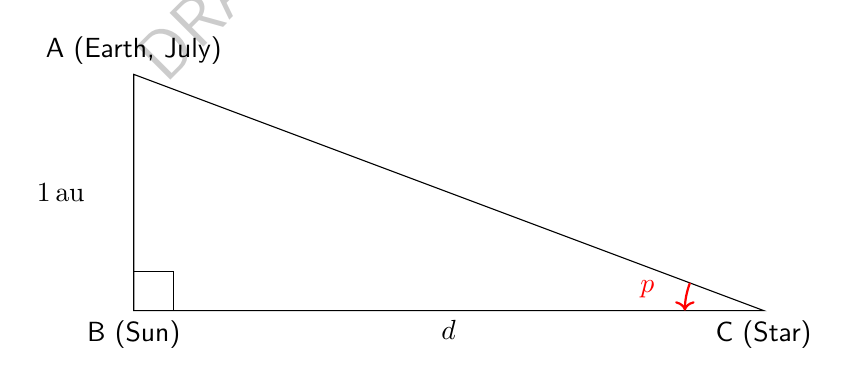
\begin{tikzpicture}
            \draw (0,0)
            coordinate (B) -- (0,3) coordinate (A) -- (8,0) coordinate (C) -- cycle
            pic ["$p$",draw,->,red,thick,angle radius=1cm,angle eccentricity=1.5] {angle = A--C--B};
            \node[above] at (0,3) {A (Earth, July)};
            \node[below] at (8,0) {C (Star)};
            \node[below] at (0,0) {B (Sun)};
            \node[left] at (-0.5, 1.5) {$\SI{1}{\astronomicalunit}$};
            \node[below] at (4,0) {$d$};
            \draw (0,0) rectangle (0.5,0.5);
          \end{tikzpicture}
        \end{figure}
  \item By small angle approximation, $p \approx \tan p = \dfrac{\SI{1}{\astronomicalunit}}{d}$.
  \item In parsecs, this is simply $d = \dfrac{1}{p}$.
\end{enumerate}

\subsection{Convenient Units}

Because we are dealing with \say{microscopic angles} in stellar parallax, scientists have introduced the unit of \textit{arcseconds} ($\degsym$) to measure these angles. This is defined as $\dfrac{1}{3600}$ of a degree. Similarly, the unit of \textit{arcminutes} is defined as $\dfrac{1}{60}$ of a degree.

\section{Stellar Radius}

Determining the stellar radius:
\begin{enumerate}
  \item By the Stefan-Boltzmann law, $L = 4\pi\sigma R^2T^4 = \sigma AT^4$, where $L$ is the luminosity, $R$ is the radius, and $T$ is the temperature of the star.
  \item The apparent brightness of a star is given by \hl{$b = \dfrac{L}{4\pi d^2}$}, where $d$ is the distance from the star to the observer. Note that this equation only applies to the light emitted and not reflected by the star.
  \item These quantities can be compared with those of the sun; this is helpful in questions where we are just asked to determine the quantity of a star in terms of that of the sun
        \begin{enumerate}
          \item The luminosity ratio (star:sun) is given by
                $$\frac{L}{L_{\odot}} = \frac{R^2T^4}{R^2_{\odot}T^2_{\odot}}$$
          \item The stellar radius ratio (star:sun) is given by
                $$\frac{R}{R_{\odot}} = \sqrt{\frac{L}{L_{\odot}}\frac{T_{\odot}^4}{T^4}} = \frac{T_{\odot}^2}{T^2}\sqrt{\frac{L}{L_{\odot}}}$$
          \item The apparent brightness ratio (star:sun) is given by
                $$\frac{b}{b_{\odot}} = \frac{L}{L_{\odot}}\frac{d_{\odot}^2}{d^2}$$
        \end{enumerate}
\end{enumerate}

\section{Question Bank Screenshots}

Im too lazy mate.

\img{exam/1.png}{1}{Question 1}{exam1}

\img{exam/2.png}{1}{Question 2}{exam2}
\img{exam/3.png}{1}{Question 3}{exam3}
\img{exam/4.png}{1}{Question 4}{exam4}
\img{exam/5.png}{1}{Question 5}{exam5}
\img{exam/6.png}{1}{Question 6}{exam6}
\img{exam/7.png}{1}{Question 7}{exam7}
\img{exam/8.png}{1}{Question 8}{exam8}
\img{exam/9.png}{1}{Question 9}{exam9}
\img{exam/10.png}{1}{Question 10}{exam10}
\img{exam/11.png}{1}{Question 11}{exam11}
\img{exam/12.png}{1}{Question 12}{exam12}
\img{exam/13.png}{1}{Question 13}{exam13}
\img{exam/14.png}{1}{Question 14}{exam14}
\img{exam/15.png}{1}{Question 15}{exam15}
\img{exam/16.png}{1}{Question 16}{exam16}
\img{exam/17.png}{1}{Question 17}{exam17}
\img{exam/18.png}{1}{Question 18}{exam18}
\img{exam/19.png}{1}{Question 19}{exam19}
\img{exam/20.png}{1}{Question 20}{exam20}

\pagebreak

\section{Exam Questions}

\subsection{Misc \#1}

The diagram shows the extreme positions of star A six months apart as seen from Earth. The black dots are the fixed positions of distant stars. The horizontal scale is
in arc-seconds.

\img{ex/1.png}{0.8}{Diagram}{ex1}

\begin{enumerate}[label=(\alph*)]
  \item Show that the distance to star A is about 10 pc.
        \begin{itemize}
          \item The key is to understand that the horizontal axis of the diagram is twice the parallax angle $p$.
                \begin{align*}
                  p & = \dfrac{1}{2}\Delta \theta      \\
                    & = \dfrac{1}{2}\times 0.18 = 0.09 \\
                  d & = \dfrac{1}{p}                   \\
                    & = \dfrac{1}{0.09}                \\
                    & = 11.1 \text{ pc}
                \end{align*}
        \end{itemize}
  \item Calculate the ratio $\dfrac{\text{distance to star A}}{\text{distance from Earth to Sun}}$
        \begin{itemize}
          \item Essentially we are trying to compute
                $$\frac{11 \text{ pc}}{1 \text{ AU}}$$
          \item We know that $1 \text{ pc} = 206265 \text{ AU}$, so
                $$\frac{11 \text{ pc}}{1 \text{ AU}} = \frac{11 \times 206265 \text{ AU}}{1 \text{ AU}} = 2.27\times 10^6$$
        \end{itemize}
  \item The analysis of the stellar spectrum of star B shows that it has a surface temperature of 9900 K. Star B is a main sequence star with a luminosity of 25$L_\odot$, where $L_\odot$ is the luminosity of the Sun.
        \begin{enumerate}[label=(\roman*)]
          \item Outline how the temperature of a star can be determined from its stellar spectrum.
                \begin{itemize}
                  \item Identify the peak wavelength $\lambda_{\max}$
                  \item The temperature can be found with Wien's law, $\lambda_{\max}T = b$, where $b =  2.9\times 10^{-3}$.
                \end{itemize}
        \end{enumerate}

\end{enumerate}

\pagebreak

\subsection{Misc \#2}

The parallax angle of the starVega is 0.131 arc seconds.

\begin{enumerate}[label=(\alph*)]
  \item Show that the distance to Vega is 25 light years.
        \begin{itemize}
          \item The distance in parsecs is given by $d = \dfrac{1}{p}$, where $p$ is the parallax angle in arc seconds.
                \begin{align*}
                  d & = \dfrac{1}{0.131} \\
                    & = 7.63 \text{ pc}
                \end{align*}
          \item To convert to light years, we use the conversion factor $1 \text{ pc} = 3.26 \text{ light years}$.
                \begin{align*}
                  d & = 7.63 \times 3.26         \\
                    & = 24.9 \text{ light years}
                \end{align*}
        \end{itemize}
  \item The following information is available for the stars Vega and Ori.
        \img{ex/2.png}{0.6}{Table of stars}{ex2}
        \begin{enumerate}[label=(\roman*)]
          \item Determine whether Vega or $\beta$ Ori appears brighter from Earth.
                \begin{itemize}
                  \item We calculate the ratios of the apparent brightness of the two stars.
                        \begin{align*}
                          \frac{b_{\text{Vega}}}{b_{\beta \text{Ori}}} & = \frac{L_{\text{Vega}}}{L_{\beta \text{Ori}}}\frac{d_{\beta \text{Ori}}^2}{d_{\text{Vega}}^2} \\
                                                                       & = \frac{54L_\odot}{40000L_\odot}\frac{(780)^2}{(25)^2} = 1.3                                   \\
                          \implies b_{\text{Vega}}                     & > b_{\beta \text{Ori}}
                        \end{align*}

                \end{itemize}
          \item Calculate the ratio $\dfrac{\text{radius of } \beta}{\text{radius of Vega}}$
                \begin{align*}
                  \frac{L_\beta}{L_V} = \frac{R_\beta^2T_\beta^4}{R_V^2T_V^4} & \implies \frac{40000}{54} =  \left(\frac{R_\beta}{R_V}\right)^2\left(\frac{11000}{9600}\right)^4 \\\frac{ R_\beta}{R_V} &=21
                \end{align*}
        \end{enumerate}

  \item
        \begin{enumerate}[label=(\roman*)]
          \item Discuss whether $\beta$ Ori is a main sequence star.
                \begin{itemize}
                  \item No, because it has a similar temperature to that of Vega (which is a main sequence star) but a much larger luminosity.
                \end{itemize}
          \item Describe the most likely final stage in the evolution of Vega.
                \begin{itemize}
                  \item Vega is a low mass star, so it will go through red giant phase.
                  \item It will then evolve to become a white dwarf, a very small/dense/hot/dead/low luminosity star.

                \end{itemize}
        \end{enumerate}

\end{enumerate}

\pagebreak

\subsection{Conservation of Momentum}

The following reaction represents a nuclear fusion reaction:

$$\atom{2}{1}{H} + \atom{2}{1}{H} \rightarrow \atom{3}{2}{He} +  n$$

The following data is given about the reaction:
\begin{itemize}
  \item The mass of $\atom{2}{1}{H}$ is 2.014u.
  \item The mass of $\atom{3}{2}{He}$ is 3.016u.
\end{itemize}

All the energy released from the reaction goes into kinetic energy. Assume that both of the $\atom{2}{1}{H}$ particles are initially at rest. Determine the speed of the neutron. \hfill [6]

\begin{itemize}
  \item This question is a standard momentum + energy conservation question.
  \item We first calculate the energy released from the reaction.
        \begin{align*}
          \Delta m & = 2\atom{2}{1}{H} - \atom{3}{2}{He} - n                      \\
                   & = 0.0033 \text{u}                                            \\
          E        & = 0.0033 \times 931.5                   = 3.07 \si{\mega\eV}
        \end{align*}
  \item This energy is conserved, which means
        $$3.07 \si{\mega\eV} = \frac{1}{2}\left(m_nv_n^2 + (2m_p + m_n)v_H^2\right)$$
  \item We also have the conservation of momentum, so $$0 = p_n + p_H \iff m_nv_n = -(2m_p + m_n)v_H$$
  \item The values of $m_p$ and $m_n$ are given in the formula booklet, so this becomes a system of equations about $v_n$ and $v_H$.
\end{itemize}

\pagebreak

\end{document}